\subsection{Planar coils}
As PCBs are 2D objects we can't work on the z-axis to create the coil's windings. This means that the windings have to be created on the same plane. 
In 1984 researchers from Osaka University proposed the first implementation of a possible solution in the form of planar coils.
They proposed and tested a structure comprised of concentric spirals, with different shapes, made of a conductive material (mostly copper) suspended in an insulation material and then covered by two magnetic material layers \textcolor{red}{(???)}\cite{OG_plan_coils}. % TODO: Check this "magnetic material layers" part

\begin{figure}
    \centering
    \resizebox{.8\linewidth}{!}{\includesvg[draft = false, width = 1\textwidth]{Chapters/Chapter2/PCB_coils/Figures/planar_coil.svg}}
    \caption{Internal structure of a planar coil.}
    \label{fig:Planar_coil_structure}
\end{figure}

%(spiega i layers)

With the mainstream adoption of PCBs in the electronics industry, researchers have created planar coils using PCBs by etching spiral patterns on the copper layer. This allowed for the production of planar coils easily and cheaply.

The main advantage of planar coils is that they can be easily integrated into the PCB design, reducing the overall size of the device. This is particularly useful in the case of wireless power transfer systems, where the coils are used to transfer power between devices. The smaller size of the coils allows for more compact and portable devices.

Another advantage is the ability to design coils of arbitrary shapes and sizes, depending on the requirements of the application. This flexibility allows for the creation of coils that are optimized for specific applications and PCB shapes, resulting in improved performance.

\begin{figure}[th]
    \centering
    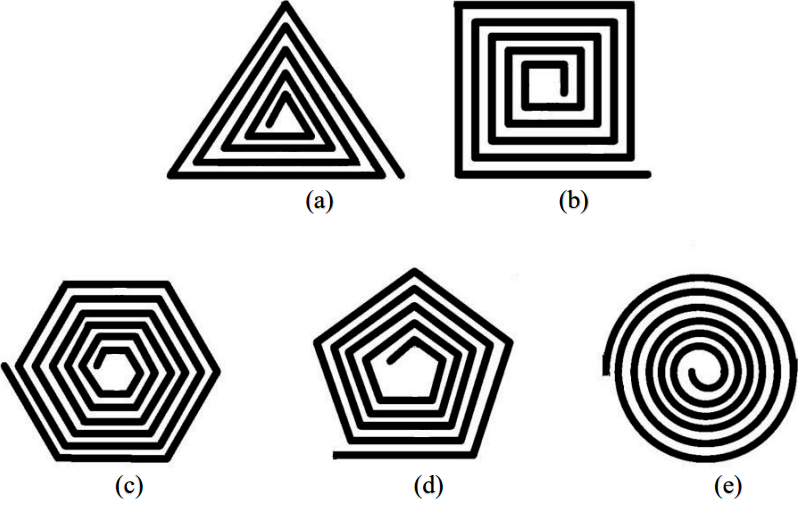
\includegraphics[scale=0.4]{Chapters/Chapter2/PCB_coils/Figures/coils_shapes.png}
    \caption[Coils Shapes]{Different planar coil architectures such as (a) triangle, (b) square, (c)
    pentagon, (d) hexagon, (e) circle.}
    \label{fig:Coils Shapes}
\end{figure}